\section{Introduction}

\subsection{Motivation}

\begin{frame}{Motivation}
  \begin{figure}
    \begin{center}
      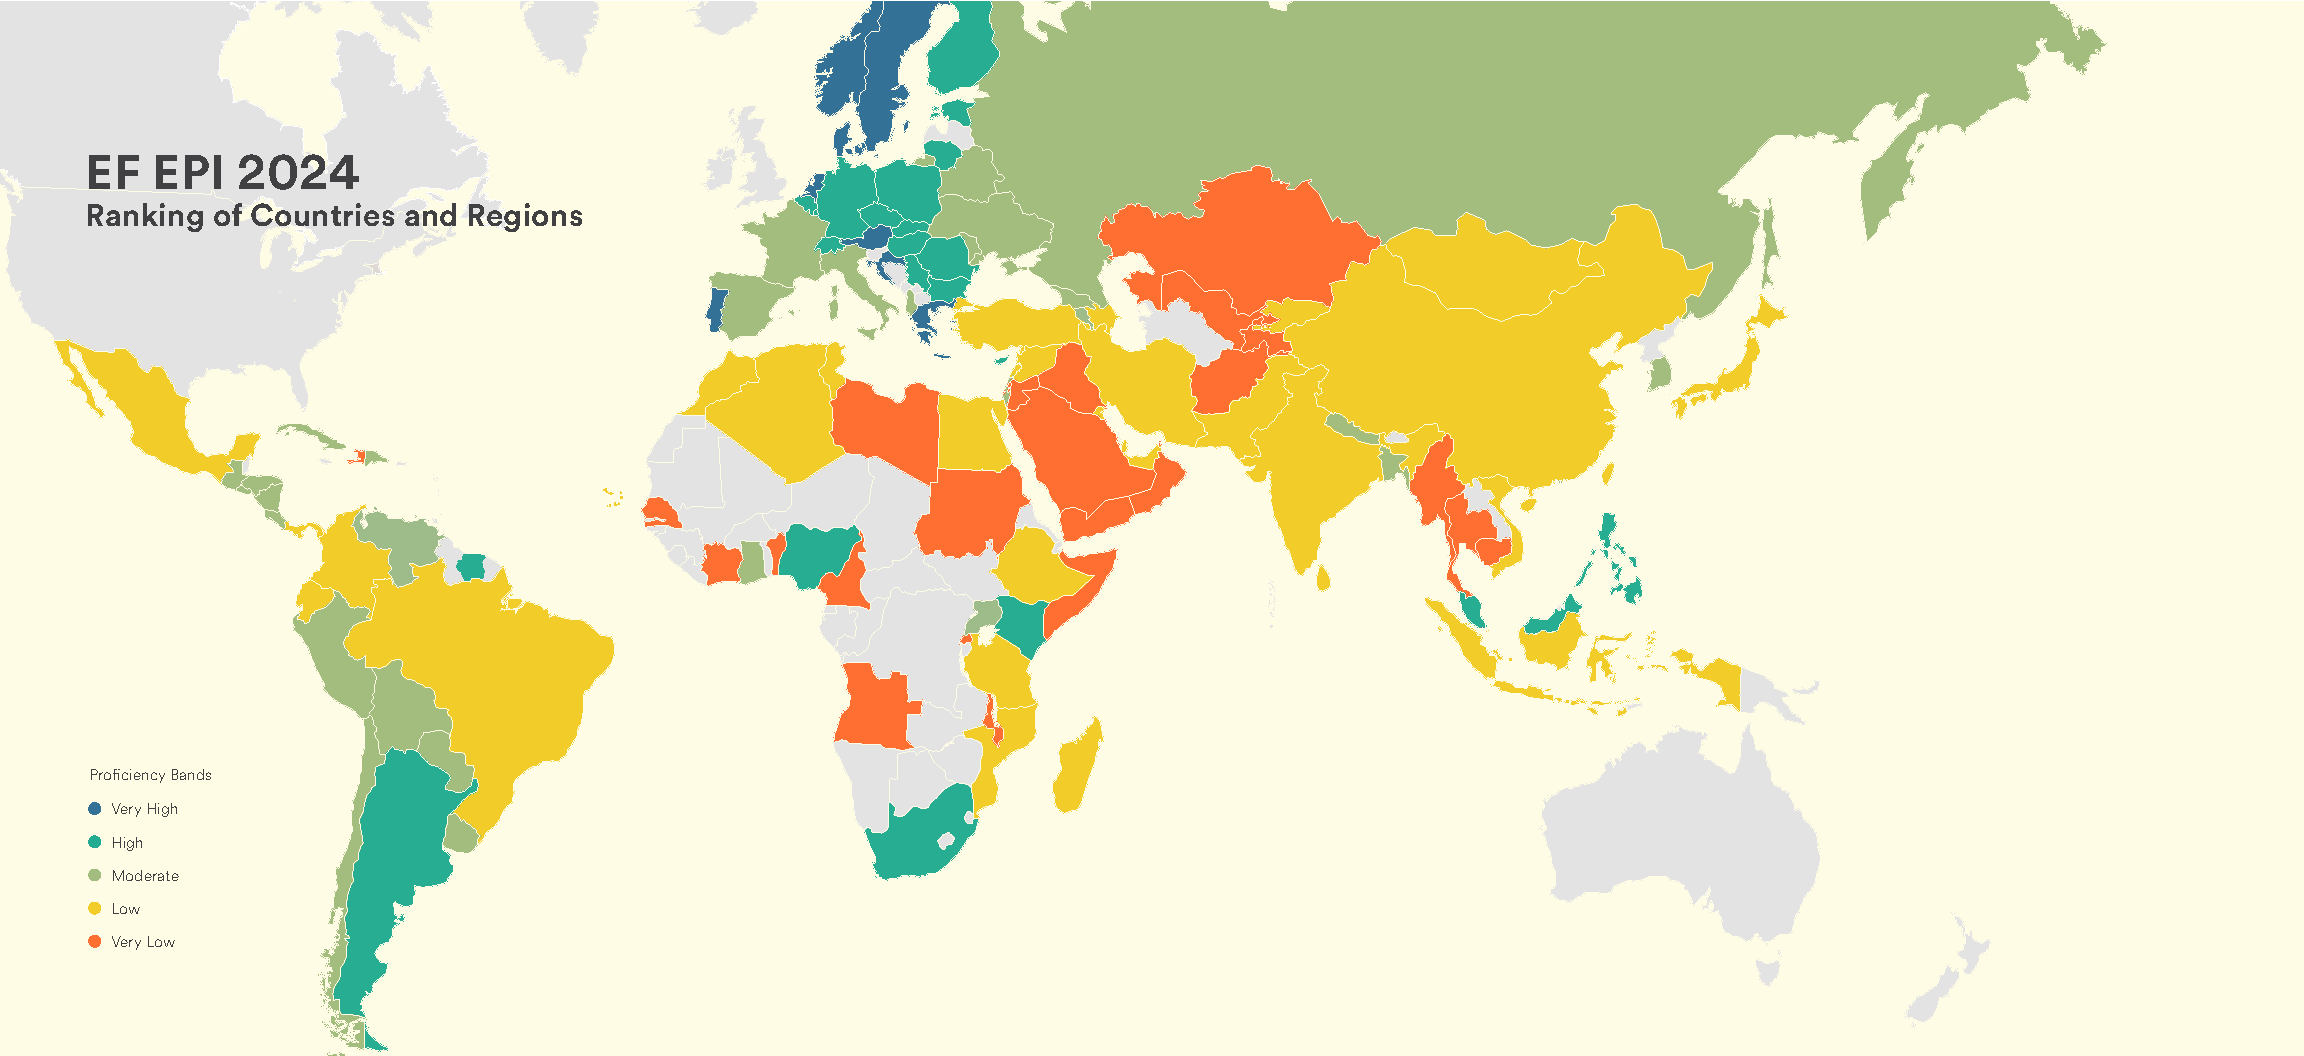
\includegraphics[width=\textwidth]{figures/ef-epi-2024-english-crop.pdf}
      \begin{textblock*}{8cm}(\paperwidth-9cm, \paperheight-2cm)  % (x,y) coordinates from top-left
        \textbf{\Large $> 1.4$ billion speakers}

        \textbf{\Large $\sim 75\%$ non-native}
      \end{textblock*}
    \end{center}
    \caption{English Proficiency bands by countries 2024 report}\label{fig:ef-epi}
  \end{figure}
\end{frame}

\note{
  English is one of the most widely used languages globally, serving as a common medium of communication for over 1.4 billion people worldwide, with almost 75\% of them being non-native speakers.
  As the number of esl and efl learners continues to grow, the demand for effective language learning tools and resources has increased significantly.
  However, grammatical and spelling errors remain common challenges for many writers, affecting clarity and professionalism.
}

% \begin{frame}{Motivation}
%   English is one of the most widely used languages globally, serving as a common medium of communication for over \alert{1.4 billion} people worldwide, with almost \alert{75\%} of them being non-native speakers~\citep{eberhard2015ethnologue}.
%   As the number of esl and efl learners continues to grow, the demand for effective language learning tools and resources has increased significantly.
%   However, grammatical and spelling errors remain common challenges for many writers, affecting clarity and professionalism.
% \end{frame}
